\documentclass{article}

\usepackage{pgfplots}
\usepgfplotslibrary{groupplots}
\usepackage{xcolor}
\definecolor{azul}{rgb}{0.0, 0.0, 0.55}

\begin{document}

%%%%%%%%%%%%%%%%%%
% SIN COLOR %
%%%%%%%%%%%%%%%%%%


%%%%%%%%%%%%%%%%%%%
% FIGURE 1 %
%%%%%%%%%%%%%%%%%%%

\makebox[\textwidth][c]{
\begin{tikzpicture}[scale=1]
\begin{groupplot}[
    group style = {group size=2 by 1},
    ymin=-0.05, ymax=0.2, xmin=-0.05, xmax=0.3,
    ylabel = {$f(P),K(d)$},
    axis y line=middle,  axis x line=middle,
    axis line style={latex-latex},
    ytick={0.065,0.1,0.125}, yticklabels=\empty,
    scale=1.3 ]

%Gráfico de la izquierda
\nextgroupplot[xlabel = $P$, xtick={0.0059,0.0191,0.0625,0.1309,0.1791}, xticklabels=\empty]
\addplot [ domain=0:0.28, samples=100 ]  {x^(1/2) - 2*x} node[left] {$f(P)$};
\addplot[domain=0:0.25]{0.1};
\addplot[domain=0:0.25]{0.065};

\draw (axis cs:0,0.125) node[left]{$\frac{R}{4k}$};
\draw (axis cs:0,0.1) node[left]{$K(0)$};
\draw (axis cs:0,0.065) node[left]{$K(d_+)$};
\draw [dotted] (axis cs:0.0625,0.125) -- (axis cs:0.0625,0) node[below]{$\frac{R^2}{4k^2}$};
\draw [dotted] (axis cs:0.0191,0.1) -- (axis cs:0.0191,0) node[below]{$P_1$};
\draw [dotted] (axis cs:0.1309,0.1) -- (axis cs:0.1309,0) node[below]{$P_2$};
\draw [dotted] (axis cs:0.0059,0.065) -- (axis cs:0.0059,0) node[below]{$P_3$};
\draw [dotted] (axis cs:0.1791,0.065) -- (axis cs:0.1791,0) node[below]{$P_4$};

\coordinate (izq1) at (axis cs:0,0.125);
\coordinate (izq2) at (axis cs:0.25,0.1);
\coordinate (izq3) at (axis cs:0.25,0.065);

%Gráfico de la derecha
\nextgroupplot[	xlabel = $d$, xmax=0.15, axis equal image,
    xtick={-0.025,0.035}, xticklabels=\empty]
\addplot [ domain=-0.03:0.13 ] {0.1-x} node[above=0.32cm]{$K(d)$};

\draw [dotted] (axis cs:-0.025,0.125) -- (axis cs:-0.025,0);
\draw [dotted] (axis cs:0.035,0.065) -- (axis cs:0.035,0) node[below]{$d_+$};
\coordinate (der1) at (axis cs:0,0.125);
\coordinate (der2) at (axis cs:0,0.1);
\coordinate (der3) at (axis cs:0.035,0.065);
\coordinate (nodo1) at (axis cs:0.005,0.125);
\coordinate (nodo2) at (axis cs:-0.005,0.1);
\coordinate (nodo3) at (axis cs:-0.005,0.065);
\coordinate (nodo4) at (axis cs:-0.025,-0.003);


\end{groupplot}
\draw [dotted] (izq1) -- (der1);
\draw [dotted] (izq2) -- (der2);
\draw [dotted] (izq3) -- (der3);
\draw (nodo1) node[right,fill=white]{$\frac{R}{4k}$};
\draw (nodo2) node[left,fill=white]{$y_{lb}(R+k)$};
\draw (nodo3) node[left,fill=white]{$K(d_+)$};
\draw (nodo4) node[below,fill=white]{$y_{lb}\frac{R+k}{R}-\frac{1}{4k}$}

\end{tikzpicture}
}

\vspace{2cm}

%%%%%%%%%%%%%%%%%%%
% FIGURE 2 %
%%%%%%%%%%%%%%%%%%%

\makebox[\textwidth][c]{
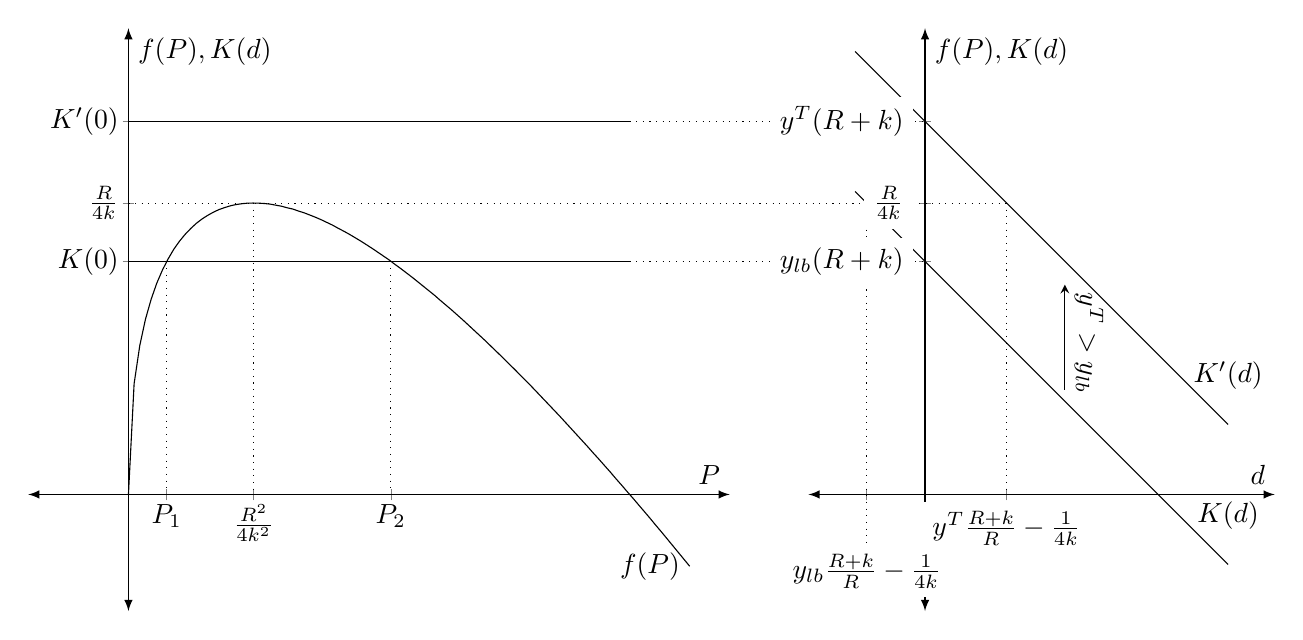
\begin{tikzpicture}[scale=1]
\begin{groupplot}[
    group style = {group size=2 by 1},
    ymin=-0.05, ymax=0.2, xmin=-0.05, xmax=0.3,
    ylabel = {$f(P),K(d)$},
    axis y line=middle,  axis x line=middle,
    axis line style={latex-latex},
    ytick={0.1,0.125,0.16}, yticklabels=\empty,
    scale=1.3 ]

%Gráfico de la izquierda
\nextgroupplot[	xlabel = $P$,
    xtick={0.0191,0.0625,0.1309}, xticklabels=\empty]
\addplot [ domain=0:0.28, samples=100 ]  {x^(1/2) - 2*x} node[left] {$f(P)$};
\addplot[domain=0:0.25]{0.16};
\addplot[domain=0:0.25]{0.1};

\draw (axis cs:0,0.125) node[left]{$\frac{R}{4k}$};
\draw (axis cs:0,0.1) node[left]{$K(0)$};
\draw (axis cs:0,0.16) node[left]{$K'(0)$};
\draw [dotted] (axis cs:0.0625,0.125) -- (axis cs:0.0625,0) node[below]{$\frac{R^2}{4k^2}$};
\draw [dotted] (axis cs:0.0191,0.1) -- (axis cs:0.0191,0) node[below]{$P_1$};
\draw [dotted] (axis cs:0.1309,0.1) -- (axis cs:0.1309,0) node[below]{$P_2$};


\coordinate (izq1) at (axis cs:0,0.125);
\coordinate (izq2) at (axis cs:0.25,0.1);
\coordinate (izq3) at (axis cs:0.25,0.16);

%Gráfico de la derecha
\nextgroupplot[	xlabel = $d$, xmax=0.15, axis equal image,
    xtick={-0.025,0.035}, xticklabels=\empty]
\addplot [ domain=-0.03:0.13 ] {0.16-x} node[above=0.32cm]{$K'(d)$};
\addplot [ domain=-0.03:0.13 ] {0.1-x} node[above=0.32cm]{$K(d)$};


\draw [dotted] (axis cs:0.035,0.125) -- (axis cs:0.035,0);
\draw [dotted] (axis cs:-0.025,0.125) -- (axis cs:-0.025,-0.025);
\draw [->,>=stealth] (axis cs:0.06,0.045) -- (axis cs:0.06,0.09);
\draw (axis cs:0.06,0.065) node[above,rotate=-90]{$y^T>y_{lb}$};
\coordinate (der1) at (axis cs:0.035,0.125);
\coordinate (der2) at (axis cs:0,0.1);
\coordinate (der3) at (axis cs:0,0.16);
\coordinate (nodo1) at (axis cs:-0.005,0.125);
\coordinate (nodo2) at (axis cs:-0.005,0.16);
\coordinate (nodo3) at (axis cs:-0.005,0.1);
\coordinate (nodo4) at (axis cs:0.035,-0.003);
\coordinate (nodo5) at (axis cs:-0.025,-0.0215);

\end{groupplot}
\draw [dotted] (izq1) -- (der1);
\draw [dotted] (izq2) -- (der2);
\draw [dotted] (izq3) -- (der3);
\draw (nodo1) node[left,fill=white]{$\frac{R}{4k}$};
\draw (nodo2) node[left,fill=white]{$y^T(R+k)$};
\draw (nodo3) node[left,fill=white]{$y_{lb}(R+k)$};
\draw (nodo4) node[below,fill=white]{$y^T\frac{R+k}{R}-\frac{1}{4k}$};
\draw (nodo5) node[below,fill=white]{$y_{lb}\frac{R+k}{R}-\frac{1}{4k}$};

\end{tikzpicture}
}

\newpage
%%%%%%%%%%%%%%%%%%
% CON COLOR %
%%%%%%%%%%%%%%%%%%


%%%%%%%%%%%%%%%%%%%
% FIGURE 1 %
%%%%%%%%%%%%%%%%%%%

\makebox[\textwidth][c]{
\begin{tikzpicture}[scale=1]
\begin{groupplot}[
    group style = {group size=2 by 1},
    ymin=-0.05, ymax=0.2, xmin=-0.05, xmax=0.3,
    ylabel = {$f(P),K(d)$},
    axis y line=middle,  axis x line=middle,
    axis line style={latex-latex},
    ytick={0.065,0.1,0.125}, yticklabels=\empty,
    scale=1.3 ]

%Gráfico de la izquierda
\nextgroupplot[xlabel = $P$,
    xtick={0.0059,0.0191,0.0625,0.1309,0.1791}, xticklabels=\empty]
\addplot [ domain=0:0.28, samples=100, red]  {x^(1/2) - 2*x} node[left] {$f(P)$};
\addplot[domain=0:0.25,blue]{0.1};
\addplot[domain=0:0.25,azul]{0.065};

\draw (axis cs:0,0.125) node[left,red]{$\frac{R}{4k}$};
\draw (axis cs:0,0.1) node[left,blue]{$K(0)$};
\draw (axis cs:0,0.065) node[left]{$K(d_+)$};
\draw [dotted,red] (axis cs:0.0625,0.125) -- (axis cs:0.0625,0) node[below,red]{$\frac{R^2}{4k^2}$};
\draw [dotted,blue] (axis cs:0.0191,0.1) -- (axis cs:0.0191,0) node[below,blue]{$P_1$};
\draw [dotted,blue] (axis cs:0.1309,0.1) -- (axis cs:0.1309,0) node[below,blue]{$P_2$};
\draw [dotted] (axis cs:0.0059,0.065) -- (axis cs:0.0059,0) node[below]{$P_3$};
\draw [dotted] (axis cs:0.1791,0.065) -- (axis cs:0.1791,0) node[below]{$P_4$};

\coordinate (izq1) at (axis cs:0,0.125);
\coordinate (izq2) at (axis cs:0.25,0.1);
\coordinate (izq3) at (axis cs:0.25,0.065);

%Gráfico de la derecha
\nextgroupplot[	xlabel = $d$, xmax=0.15, axis equal image,
    xtick={-0.025,0.035}, xticklabels=\empty]
\addplot [domain=-0.03:0.13, blue] {0.1-x} node[above=0.32cm]{$K(d)$};

\draw [dotted,red] (axis cs:-0.025,0.125) -- (axis cs:-0.025,0);
\draw [dotted] (axis cs:0.035,0.065) -- (axis cs:0.035,0) node[below]{$d_+$};
\coordinate (der1) at (axis cs:0,0.125);
\coordinate (der2) at (axis cs:0,0.1);
\coordinate (der3) at (axis cs:0.035,0.065);
\coordinate (nodo1) at (axis cs:0.005,0.125);
\coordinate (nodo2) at (axis cs:-0.005,0.1);
\coordinate (nodo3) at (axis cs:-0.005,0.065);
\coordinate (nodo4) at (axis cs:-0.025,-0.003);


\end{groupplot}
\draw [dotted,red] (izq1) -- (der1);
\draw [dotted,blue] (izq2) -- (der2);
\draw [dotted] (izq3) -- (der3);
\draw (nodo1) node[right,fill=white]{$\frac{R}{4k}$};
\draw (nodo2) node[left,blue,fill=white]{$y_{lb}(R+k)$};
\draw (nodo3) node[left,fill=white]{$K(d_+)$};
\draw (nodo4) node[below,red,fill=white]{$y_{lb}\frac{R+k}{R}-\frac{1}{4k}$}

\end{tikzpicture}
}

\vspace{2cm}

%%%%%%%%%%%%%%%%%%%
% FIGURE 2 %
%%%%%%%%%%%%%%%%%%%

\makebox[\textwidth][c]{
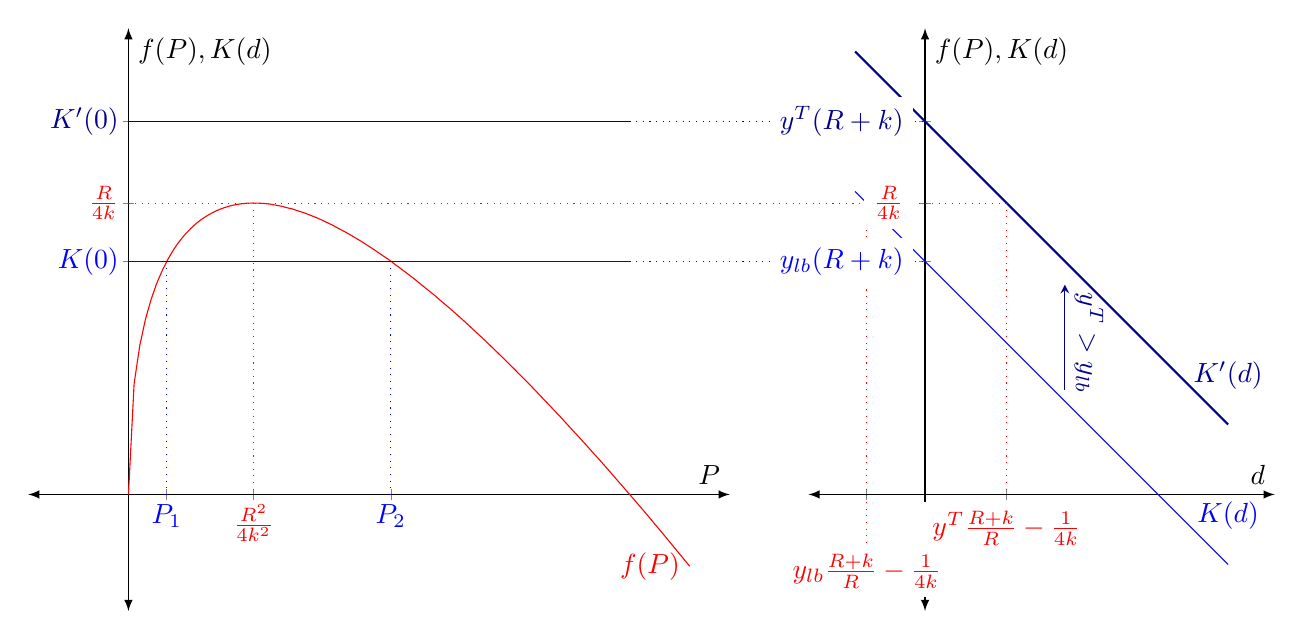
\begin{tikzpicture}[scale=1]
\begin{groupplot}[
    group style = {group size=2 by 1},
    ymin=-0.05, ymax=0.2, xmin=-0.05, xmax=0.3,
    ylabel = {$f(P),K(d)$},
    axis y line=middle,  axis x line=middle,
    axis line style={latex-latex},
    ytick={0.1,0.125,0.16}, yticklabels=\empty,
    scale=1.3 ]

%Gráfico de la izquierda
\nextgroupplot[	xlabel = $P$,
    xtick={0.0191,0.0625,0.1309}, xticklabels=\empty]
\addplot [domain=0:0.28, samples=100, red]  {x^(1/2) - 2*x} node[left] {$f(P)$};
\addplot[domain=0:0.25,azul]{0.16};
\addplot[domain=0:0.25,blue]{0.1};

\draw (axis cs:0,0.125) node[left,red]{$\frac{R}{4k}$};
\draw (axis cs:0,0.1) node[left,blue]{$K(0)$};
\draw (axis cs:0,0.16) node[left,azul]{$K'(0)$};
\draw [dotted,red] (axis cs:0.0625,0.125) -- (axis cs:0.0625,0) node[below,red]{$\frac{R^2}{4k^2}$};
\draw [dotted,blue] (axis cs:0.0191,0.1) -- (axis cs:0.0191,0) node[below,blue]{$P_1$};
\draw [dotted,blue] (axis cs:0.1309,0.1) -- (axis cs:0.1309,0) node[below,blue]{$P_2$};


\coordinate (izq1) at (axis cs:0,0.125);
\coordinate (izq2) at (axis cs:0.25,0.1);
\coordinate (izq3) at (axis cs:0.25,0.16);

%Gráfico de la derecha
\nextgroupplot[	xlabel = $d$, xmax=0.15, axis equal image,
    xtick={-0.025,0.035}, xticklabels=\empty]
\addplot [domain=-0.03:0.13, azul,thick] {0.16-x} node[above=0.32cm]{$K'(d)$};
\addplot [domain=-0.03:0.13, blue] {0.1-x} node[above=0.32cm]{$K(d)$};


\draw [dotted,red] (axis cs:0.035,0.125) -- (axis cs:0.035,0);
\draw [dotted,red] (axis cs:-0.025,0.125) -- (axis cs:-0.025,-0.025);
\draw [->,>=stealth,azul] (axis cs:0.06,0.045) -- (axis cs:0.06,0.09);
\draw (axis cs:0.06,0.065) node[above,rotate=-90,azul]{$y^T>y_{lb}$};
\coordinate (der1) at (axis cs:0.035,0.125);
\coordinate (der2) at (axis cs:0,0.1);
\coordinate (der3) at (axis cs:0,0.16);
\coordinate (nodo1) at (axis cs:-0.005,0.125);
\coordinate (nodo2) at (axis cs:-0.005,0.16);
\coordinate (nodo3) at (axis cs:-0.005,0.1);
\coordinate (nodo4) at (axis cs:0.035,-0.003);
\coordinate (nodo5) at (axis cs:-0.025,-0.0215);

\end{groupplot}
\draw [dotted,red] (izq1) -- (der1);
\draw [dotted,blue] (izq2) -- (der2);
\draw [dotted,azul] (izq3) -- (der3);
\draw (nodo1) node[left,red,fill=white]{$\frac{R}{4k}$};
\draw (nodo2) node[left,azul,fill=white]{$y^T(R+k)$};
\draw (nodo3) node[left,blue,fill=white]{$y_{lb}(R+k)$};
\draw (nodo4) node[below,red,fill=white]{$y^T\frac{R+k}{R}-\frac{1}{4k}$};
\draw (nodo5) node[below,red,fill=white]{$y_{lb}\frac{R+k}{R}-\frac{1}{4k}$};

\end{tikzpicture}
}



\end{document}
